\section{Photon number calibration}

In the previous section, we showed how to measure the resonator photon number using the ac Stark shift.
We used Eq.\,\ref{eq:ch:results:sec:characterization:acStarckShift} to convert a time resolved measurement of $\delta \omega_{10}$ to a time resolved measurement of $n$.
We also need a calibration between resonator drive \emph{amplitude} and the steady state value of $n$.
This can be thought of as measuring the $t=100\,\text{ns}$ point of Fig.\,\ref{Fig:ch:results:sec:characterization:photonsVsTime}\,c as we vary the amplitude of the measurement resonator drive pulse.
Therefore, the pulse sequence is essentially the same as shown in Fig.\,\ref{Fig:ch:results:sec:characterization:photonsVsTime}\,a, with two differences.
\begin{enumerate}
\item The $\pi$-pulse placed at a fixed $\tau$, in the steady state part of the resonator ring up.
\item We vary the resonator drive pulse amplitude.
\end{enumerate}
This yields a measurement of the qubit frequency as a function of resonator drive amplitude, as shown in Fig.\,\ref{Fig:ch:results:sec:photonNumberCalibration:acStark}.
Assuming that the resonator internal energy is proportional to the square of the amplitude of the drive signal, we have \begin{equation}
\frac{\delta \omega_{10}}{2 \chi} = n = m A^2 . \end{equation}
With the value of $\chi$ previously, we measure the dependence of $\delta \omega_{10}$ on the drive amplitude and extract $m$.
In subsequent experiments we mapped drive amplitude to resonator photon number via $n = mA^2$.

\begin{figure}
\begin{centering}
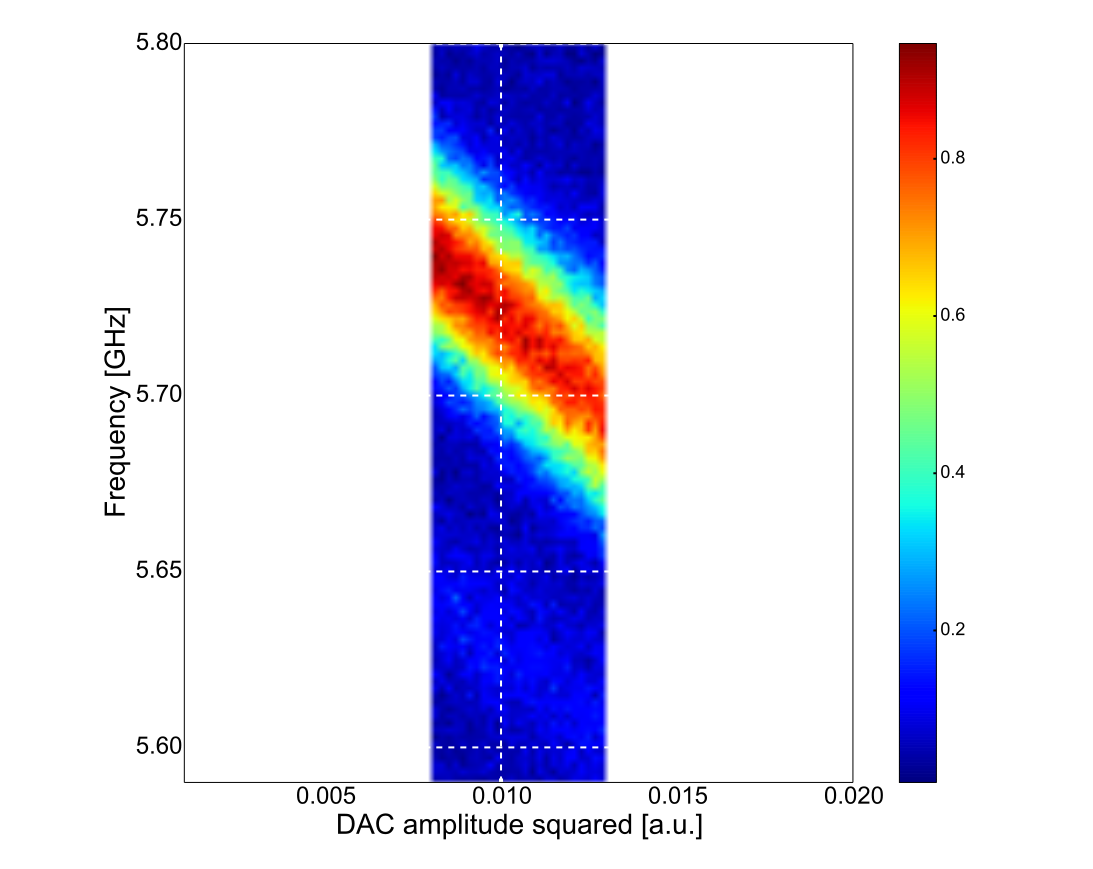
\includegraphics[width=\textwidth]{acStark.pdf}
\par\end{centering}
\caption{AC Stark shift measured via qubit detuning during measurement.}
\label{Fig:ch:results:sec:photonNumberCalibration:acStark}
\end{figure}
